\section{Core and relativistic states}\label{sec:10.6}

A germanium atom has 32 electrons, and the band structure of \cref{sec:10.1} follows four of them. Ten more sit in the $3d$ shell, \SI{29.4}{eV} below the valence-band maximum, close enough for light dark matter to excite them, and the deeper shells follow at \SI{122}{eV} and beyond. \Cref{sec:3.5} found where each shell becomes kinematically accessible and why the momenta it needs are large: an electron that absorbs $\omega$ must receive at least $q = \omega/v_{\mathrm{max}}$, \SI{11}{keV} for germanium $3d$ and \SI{38}{keV} for silicon $2p$. It left two questions for the rate. At which momentum transfer does a core shell actually take over from the valence electrons, given that both are probed far out in the tails of their momentum distributions? And how much do the relativistic corrections of order $(Z\alpha)^2$, which grow with the depth of the shell, change the response there? We answer both for silicon and germanium, and find the three hypotheses under which the response of the core electrons separates from that of the valence electrons: a filled shell, a flat band and orthogonal site orbitals.

\subsection{Core shells within kinematic reach}\label{sec:10.6-reach}

The structure factor of a crystal with core shells is the sum of the valence term of \cref{eq:10.1-S0} and one term per core shell. The core states of atom $\kappa$ in the cell are the Bloch sums $\psi_{\kappa nlm,\vect{k}}$ of \cref{eq:E.7-core}, with the energy $-E_{\mathrm{core}}$ measured from the valence maximum, and their vertex with a conduction state is $\rho_{c,\kappa nlm}(\vect{k},\vect{q}) = \langle\psi_{c,\vect{k}+\vect{q}}|\ee^{\ii\vect{q}\cdot\vect{r}}|\psi_{\kappa nlm,\vect{k}}\rangle$. Following the steps of \cref{eq:10.1-S0} with these states in place of the valence bands,
\begin{equation}
  S^0_{\mathrm{core}}(\vect{q},\omega) = 4\pi\sum_{\kappa nlm}\sum_c\int_{\mathrm{BZ}}\frac{\dd^3k}{(2\pi)^3}\,|\rho_{c,\kappa nlm}(\vect{k},\vect{q})|^2\,\delta\bigl(\omega - \varepsilon_{c,\vect{k}+\vect{q}} - E_{\mathrm{core},\kappa nl}\bigr) .
  \label{eq:10.6-core}
\end{equation}
Both states in the vertex must be all-electron states. The core orbital is all-electron by construction. The conduction state must carry its core-region oscillations, which the reconstruction \cref{eq:3.5-rhoAE} restores, because the overlap with a core orbital is taken inside the sphere where a pseudo-wavefunction is wrong. A semicore shell kept in the valence of the pseudopotential, such as germanium $3d$, enters \cref{eq:10.1-S0} instead, with reconstructed vertices on both sides. Griffin and coworkers computed the germanium $3d$ contribution both ways and found that the atomic orbitals reproduce the reconstructed crystal states up to the largest momentum the crystal calculation resolves, about \SI{45}{keV}~\cite[Sects.~2.2 and~3.3]{griffin2021extended}.

How many core electrons can dark matter reach at a given $q$? A momentum transfer $q$ deposits at most $qv_{\mathrm{max}}$, whatever the mass (\cref{eq:1.3-vmin}), so the relevant measure is the part of the structure factor below that energy. Per atom and per shell we define
\begin{equation}
  N^{\mathrm{acc}}_{nl}(q) = \int_{\Eg + E_{\mathrm{core}}}^{qv_{\mathrm{max}}}\dd\omega\;S^{\mathrm{at}}_{nl}(q,\omega) ,
  \label{eq:10.6-Nacc}
\end{equation}
where $S^{\mathrm{at}}_{nl}(q,\omega)$ is the response of one atom's shell, normalized so that its integral over all $\omega$ is the occupation $N_{nl}$ when $q$ is large (closure, \cref{sec:4.3}). The structure factor of \cref{eq:10.6-core} is $(2\pi/\Omega)\sum_\kappa S^{\mathrm{at}}_{\kappa nl}$, as the next subsection shows, so $N^{\mathrm{acc}}_{nl}$ counts the electrons of a shell, per atom, that the halo can excite at momentum transfer $q$. With plane-wave final states the shell response follows from the ionization form factor of \cref{sec:2.2}. The number of final states per unit ejected energy is $|f_{\mathrm{ion}}|^2/4E_{\mathrm{ej}}$, and \cref{eq:2.2-fion-pw}, with the radial momentum orbital $\phi_{nl}(k)$ of \cref{sec:3.5} normalized to $\int k^2\phi_{nl}^2\,\dd k = 1$, gives
\begin{equation}
  S^{\mathrm{at}}_{nl}(q,\omega) = \frac{N_{nl}}{2}\,\frac{m_e}{q}\int_{|p - q|}^{p + q}k\,\phi_{nl}(k)^2\,\dd k , \qquad p = [2m_e(\omega - E_{\mathrm{core}})]^{1/2} ,
  \label{eq:10.6-Sat}
\end{equation}
for a full shell, $N_{nl} = 2(2l + 1)$, and for the spherical average of a partly filled valence shell. The final kinetic energy is counted from the valence maximum, as for the free final states of Griffin and coworkers~\cite[Eq.~(3.21)]{griffin2021extended}. Integrating over $\omega$, with $\dd\omega = p\,\dd p/m_e$ and the order of integration exchanged, each $k$ collects $\int_{|k - q|}^{k + q}p\,\dd p = 2kq$, and the integral is $N_{nl}\int k^2\phi_{nl}^2\,\dd k = N_{nl}$: closure holds.

\Cref{eq:10.6-Sat} explains when a shell takes over. Near its opening the ejected momentum $p$ is much smaller than $q$, the integral is $2pq\,\phi_{nl}(q)^2$, and
\begin{equation*}
  N^{\mathrm{acc}}_{nl}(q) \simeq N_{nl}\,m_e\,\phi_{nl}(q)^2\int_{E_{\mathrm{core}}}^{qv_{\mathrm{max}}}p\,\dd\omega = \frac{2\sqrt2}{3}\,N_{nl}\,m_e^{3/2}\,\phi_{nl}(q)^2\,(qv_{\mathrm{max}} - E_{\mathrm{core}})^{3/2} ,
\end{equation*}
where the gap has been dropped from the lower limit. Two factors decide. The first is the number of electrons of the shell per unit volume of momentum at $p = q$, $N_{nl}\phi_{nl}(q)^2$, in which a core shell beats the valence above about \SI{5}{keV} (\cref{fig:3-core}). The second is the phase space $(qv_{\mathrm{max}} - E_{\mathrm{core}})^{3/2}$, which is zero at the opening and approaches that of the valence, $(qv_{\mathrm{max}})^{3/2}$, only once $qv_{\mathrm{max}}$ is several times $E_{\mathrm{core}}$. A core shell therefore overtakes the valence a little above its opening, at the momentum where its larger density outweighs the reduced phase space.

\Cref{fig:10-core} evaluates \cref{eq:10.6-Nacc} for germanium. The core and semicore shells use the free-atom orbitals of \cref{fig:3-core}. The valence uses the crystal: the independent-particle $\varepsilon_2$ of Knapen, Kozaczuk and Lin~\cite[Sect.~III\,B]{knapen2021dark}, from which $S = (2q^2/e^2)\varepsilon_2$ (\cref{sec:10.2}) and, per atom of the two-atom cell, $S^{\mathrm{at}} = q^2\Omega\varepsilon_2/8\pi^2\alpha$. That table holds only the four valence electrons, with the $3d$ shell frozen, on bands scissored to the measured gap at zero temperature. It ends at \SI{22.5}{keV}, where its plane-wave basis ends too, and we use it up to \SI{15}{keV} and \cref{eq:10.6-Sat} with the atomic $4s$ and $4p$ orbitals above. At the switch the two differ by 27 percent. Between 5 and \SI{15}{keV} the atomic model and the crystal tables of silicon and germanium differ by up to a factor of six in either direction, since the low-energy corner $\omega \le qv_{\mathrm{max}}$ is where the band structure matters most. That is the accuracy of the valence curve beyond the table.

\begin{figure}[tbp]
  \centering
  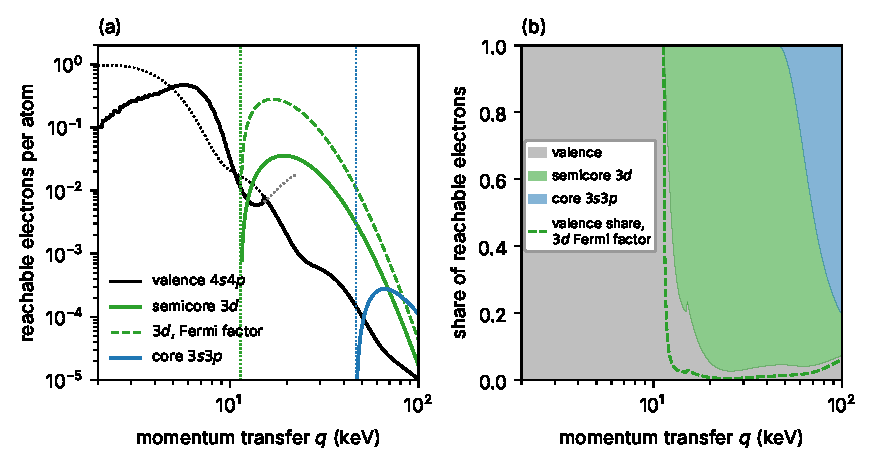
\includegraphics[width=\linewidth]{figures/ch10/fig10_5.pdf}
  \caption{Germanium electrons that dark matter of any mass can excite at momentum transfer $q$, that is, with energy deposits between the threshold of the shell and $qv_{\mathrm{max}}$, $v_{\mathrm{max}} = 2.650\times10^{-3}$. (a)~Electrons per atom, $N^{\mathrm{acc}}_{nl}(q)$ of \cref{eq:10.6-Nacc}, for the valence shell (black), the semicore $3d$ shell (green) and the core $3s$ and $3p$ shells (blue). Valence: crystal independent-particle response of Knapen, Kozaczuk and Lin (PAW, $3d$ frozen) below \SI{15}{keV}; above, the plane-wave model of \cref{eq:10.6-Sat} with the free-atom $4s$, $4p$ orbitals (dotted lines continue each curve past the switch). Core and semicore: \cref{eq:10.6-Sat} with free-atom, scalar-relativistic PBE orbitals and plane-wave final states whose kinetic energy is counted from the valence maximum; dashed, the $3d$ shell with the Fermi factor of \cref{eq:2.2-fermi} at $Z_{\mathrm{eff}} = 1$. Dotted vertical lines: the openings $(\Eg + E_{\mathrm{core}})/v_{\mathrm{max}}$ of the $3d$ and $3p$ shells, with centroid binding energies 29.4 and \SI{122.2}{eV} and $\Eg = \SI{0.744}{eV}$. Germanium $2s$, $2p$ and $1s$ open above \SI{460}{keV}. (b)~Shares of the reachable electrons: valence (gray), $3d$ (green), $3s3p$ (blue); dashed, the valence share when the $3d$ shell carries the Fermi factor. The $3d$ shell overtakes the valence at \SI{12.5}{keV} (\SI{11.5}{keV} with the Fermi factor) and holds more than 90 percent of the reachable electrons from 20 to \SI{50}{keV}.}
  \label{fig:10-core}
\end{figure}

The figure answers the first question for germanium. Below \SI{11.3}{keV} only the valence is reachable, and its count falls from 0.44 electrons per atom at \SI{5}{keV} to 0.03 at \SI{10}{keV} as the window $\omega \le qv_{\mathrm{max}}$ moves into the low-energy tail of a spectrum that is centered on $q^2/2m_e$. The $3d$ shell opens at \SI{11.3}{keV} and overtakes the valence at \SI{12.5}{keV}. By \SI{20}{keV} it holds 0.036 reachable electrons per atom against 0.002 for the valence, and it keeps more than 90 percent of the total until the $3p$ and $3s$ shells, opening at 46 and \SI{68}{keV}, take over near \SI{69}{keV}. For silicon the same model puts the opening of $2p$ at \SI{38}{keV} and its crossing with the valence at \SI{46}{keV}, and the $2s$ shell overtakes $2p$ near \SI{77}{keV}. Since the silicon valence count there comes from the atomic model, uncertain by a factor of a few, and the $2p$ count rises steeply above its opening, the crossing is uncertain by a few keV.

Two features of the model need checking, the non-orthogonality of plane-wave final states and the missing Coulomb attraction of the ion. A plane wave is not orthogonal to the bound orbital. Its projection onto the initial orbital adds a spurious term of relative size $|F_{nl}(q)|^2\phi_{nl}(p)^2/\langle\phi_{nl}(|\vect{p} - \vect{q}|)^2\rangle$, with $F_{nl}(q)$ the elastic form factor of the shell; for germanium $3d$ between 12 and \SI{30}{keV} it stays below 6 percent. The final state is the larger issue. A slow electron leaving a core region is pulled toward the ion, and the Fermi factor, 12 at a final momentum of \SI{2}{keV} and 5 at \SI{5}{keV} for $Z_{\mathrm{eff}} = 1$, raises the $3d$ count by about that much near the edge (dashed curves). This moves the crossing only from 12.5 to \SI{11.5}{keV}, because the count rises so steeply above the opening, but it changes the size of the $3d$ contribution to a rate by an order of magnitude. Crystal conduction states, as in Griffin's calculation, are the correct final states, and the Fermi factor only brackets them.

\begin{workedexample}{The germanium $3d$ onset in $q$}\label{we:10-ge3d}
The $3d$ shell is a doublet, $3d_{5/2}$ at \SI{29.2}{eV} and $3d_{3/2}$ at \SI{29.8}{eV} below the valence maximum~\cite[Table~1-1]{williams2009electron}. With $\Eg = \SI{0.744}{eV}$ the thresholds are 29.94 and \SI{30.54}{eV}, and the openings $(\Eg + E_{\mathrm{core}})/v_{\mathrm{max}}$ are \SI{11.3}{keV} and \SI{11.5}{keV}. The threshold masses $2(\Eg + E_{\mathrm{core}})/v_{\mathrm{max}}^2$ are 8.5 and \SI{8.7}{MeV}; the rounded values of \cref{sec:3.5}, \SI{11}{keV} and \SI{8.5}{MeV}, are those of a single level at \SI{29}{eV}.

Opening is not taking over. Just above \SI{11.3}{keV} the window $qv_{\mathrm{max}} - E_{\mathrm{core}}$ is a fraction of an eV wide, and the $3d$ count of \cref{eq:10.6-Nacc} starts from zero. From \cref{fig:10-core}a, at \SI{12}{keV} the $3d$ shell offers 0.0040 reachable electrons per atom against 0.0084 for the valence, at \SI{15}{keV} 0.025 against 0.0065. The two are equal at \SI{12.5}{keV} with the crystal valence. With the atomic valence the crossing is at \SI{13.1}{keV}, and with the Fermi factor on the $3d$ final states at \SI{11.5}{keV}. The onset in $q$ is therefore
\begin{equation*}
  q_{3d} \simeq (12.5 \pm 1)\,\mathrm{keV} = (3.3 \pm 0.3)\,q_0 ,
\end{equation*}
with $q_0 = \alpha m_e = \SI{3.73}{keV}$. Three quarters of the $3d$ electrons have momenta above \SI{11}{keV} (\cref{sec:3.5}), so the shell is probed near the peak of its distribution, while the valence is probed far in its tail.

Which masses use this momentum? A momentum transfer $q$ with energy deposited $\omega$ needs $\vmin = \omega/q + q/2\mchi \le v_{\mathrm{max}}$ (\cref{eq:1.3-vmin}), so at the $3d_{5/2}$ threshold, $\omega = \SI{29.94}{eV}$,
\begin{equation*}
  \mchi \ge \frac{q}{2(v_{\mathrm{max}} - \omega/q)} = \frac{\SI{12.5}{keV}}{2\,(2.650 - 2.395)\times10^{-3}} = \SI{25}{MeV} ,
\end{equation*}
and \SI{19}{MeV} for $q = \SI{13}{keV}$. A particle of \SI{10}{MeV} reaches the $3d_{5/2}$ edge only for $q$ between 16 and \SI{37}{keV}, where the $3d$ shell dominates the reachable electrons but only the fastest particles of the halo contribute, through the tail of $\eta(\vmin)$. Weighting each $(q,\omega)$ with $\eta(\vmin)$ as in the heavy-mediator rate \cref{eq:1.5-rate}, with a one-pair threshold and the valence from the crystal table below \SI{22.5}{keV} and the atomic model above, gives the ratio of the $3d$ rate to the valence rate. In the plane-wave model it is $6\times10^{-5}$ at \SI{10}{MeV}, 0.07 at \SI{30}{MeV}, 0.27 at \SI{100}{MeV} and 0.34 at \SI{1}{GeV}. With the Fermi factor it is $1\times10^{-3}$, 0.69, 2.1 and 3.4. Griffin and coworkers, with crystal conduction states, find the $3d$ term dominant for a heavy mediator above about \SI{30}{MeV} at a one-pair threshold, and at lower masses for higher thresholds~\cite[Sect.~4.1]{griffin2021extended}. The onset in $q$ is robust to the final state; the mass at which the $3d$ shell dominates the rate is not, and only a calculation with crystal final states fixes it.
\end{workedexample}

\subsection{Separation of core and valence responses}\label{sec:10.6-factor}

The core term \cref{eq:10.6-core} is a double sum over $\vect{k}$ and the orbitals $m$ of every atom, and one might expect interference between the orbitals of neighboring atoms, with phases $\ee^{\ii\vect{q}\cdot(\vect{\tau}_\kappa - \vect{\tau}_{\kappa'})}$. There is none, under three conditions. First, the shell is completely filled. Second, its band is flat on the scale of the energies that the response resolves, so that all its states share one energy $-E_{\mathrm{core}}$. Third, the atomic orbitals of different sites are orthogonal. For a final state $|f\rangle$ the sum over the initial states of the shell is then $\sum_i|\langle f|\ee^{\ii\vect{q}\cdot\vect{r}}|i\rangle|^2 = \langle f|\ee^{\ii\vect{q}\cdot\vect{r}}P_{nl}\ee^{-\ii\vect{q}\cdot\vect{r}}|f\rangle$, with $P_{nl}$ the projector on the shell. A projector does not depend on the basis that spans it, and in the basis of the atomic orbitals $\psi^{\mathrm{at}}_{\vect{R}\kappa nlm}$ of \cref{eq:E.7-core}, centered on the atom $\kappa$ of cell $\vect{R}$, it is $\sum_{\vect{R}\kappa m\sigma}|\psi^{\mathrm{at}}_{\vect{R}\kappa nlm}\sigma\rangle\langle\psi^{\mathrm{at}}_{\vect{R}\kappa nlm}\sigma|$. The sum over initial states is a sum of squares, one per site, with no cross terms. Every cell gives the same contribution by translation symmetry, and dividing by the volume,
\begin{keyresult}[Core response of a crystal]
For a filled, flat core shell with orthogonal site orbitals,
\begin{equation}
  \begin{gathered}
  S^0_{\mathrm{core}}(\vect{q},\omega) = \frac{2\pi}{\Omega}\sum_\kappa S^{\mathrm{at}}_{\kappa nl}(\vect{q},\omega), \\
  S^{\mathrm{at}}_{\kappa nl}(\vect{q},\omega) = \sum_{m,\sigma}\sum_f\bigl|\langle f|\ee^{\ii\vect{q}\cdot\vect{r}}|\psi^{\mathrm{at}}_{\kappa nlm}\sigma\rangle\bigr|^2\,\delta(\omega - \varepsilon_f - E_{\mathrm{core}}) ,
  \end{gathered}
  \label{eq:10.6-proj}
\end{equation}
the response of one site's shell to final states $|f\rangle$ of the crystal, at energies $\varepsilon_f$ above the valence maximum. With plane-wave final states it is \cref{eq:10.6-Sat}.
\end{keyresult}
\noindent The core response of the crystal is the density of atoms times a single-site response, and adds to the valence response without interference, since a core hole and a valence hole are different final states. This separation is what lets a calculation take the valence from the crystal and the core shells from the atom.

The three conditions hold well for the shells the halo reaches. The germanium $3d$ orbitals have a mean radius of \SI{0.39}{\angstrom}, against a bond length of \SI{2.45}{\angstrom}, and the crystal $3d$ bands computed by Griffin and coworkers are flat to within the spread they test~\cite[Sect.~2.2]{griffin2021extended}. Flatness must be judged per spin--orbit component. The two components of the doublet lie \SI{0.6}{eV} apart, so \cref{eq:10.6-proj} applies to each $j$ separately with its own $E_{\mathrm{core}}$, and treating the shell as one level at the centroid misplaces the edge by \SI{0.3}{eV}.

The separation fails through the final state, the core hole, screening and shells that are not flat, each outside the independent-particle response. The final state comes first, where \cref{eq:10.6-proj} keeps crystal states but every practical model replaces them: the factor of ten between free and Coulomb-attracted final states found above is the largest uncertainty in the core rate. Then the core hole. The excited electron and the hole left in the $3d$ shell attract each other and the valence electrons relax around the hole. Both shift weight toward the edge, the same physics as the valence excitons of \cref{sec:10.5}. Screening is the third. The valence electrons screen the potential that excites a core electron, by $1/|\varepsilon(\vect{q},\omega)|^2$. At large $q$ the $f$-sum rule puts the valence oscillator strength near the free recoil energy $q^2/2m_e$, so that $\varepsilon - 1 \approx \omega_p^2/[(q^2/2m_e)^2 - \omega^2]$, with $\omega_p^{\mathrm{val}} = \SI{15.6}{eV}$ for the valence electrons of germanium. At \SI{12}{keV}, where $q^2/2m_e = \SI{141}{eV}$, this is 0.012, and macroscopic screening changes the core response by about 2 percent. Local fields are less certain. For the valence response \cref{sec:10.2} found a suppression that persists at two to three times $|\vect{G}_{111}|$, and nothing comparable has been computed for core transitions. That uncertainty belongs with the many-body nuisances of \cref{sec:8.8}. The last is a shell that is not flat. A semicore shell kept in the valence hybridizes with the valence bands, and its contribution is then part of \cref{eq:10.1-S0} rather than a separate term; the separation still holds for the total, but the split between ``valence'' and ``semicore'' becomes a matter of bookkeeping.

\subsection{Relativistic corrections to the core response}\label{sec:10.6-rel}

A target described by the Dirac equation couples to dark matter through bilinears $\bar\psi\Gamma\psi\,\ee^{\ii\vect{q}\cdot\vect{r}}$. The Foldy--Wouthuysen transformation of \cref{app:C.15} turns each into nonrelativistic operators plus corrections in powers of $1/m_e$, acting on the positive-energy states. Two kinds of correction follow. The operators change, which is the picture change of the vertex. And the states change, through the mass--velocity, Darwin and spin--orbit terms of \cref{eq:3.5-HBP}.

The density vertex is the time component $\bar\psi\gamma^0\psi = \psi^\dagger\psi$, and to order $1/m_e^2$ its transform is \cref{eq:C.15-vertex}, $\ee^{\ii\vect{q}\cdot\vect{r}}[1 - q^2/8m_e^2 + (\ii/4m_e^2)\boldsymbol{\sigma}\cdot(\vect{q}\times\vect{p})]$. The scalar factor multiplies every matrix element and changes $|\rho|^2$ by $-q^2/4m_e^2$: $1.2\times10^{-4}$ at the germanium $3d$ opening, $8.6\times10^{-4}$ at \SI{30}{keV}, $2.0\times10^{-3}$ at the silicon $2p$ crossing at \SI{46}{keV}. The spin term has amplitude $qp/4m_e^2$. With the root-mean-square momentum of the germanium $3d$ shell, $p = \SI{20.4}{keV}$, it is $5.9\times10^{-4}$ at \SI{30}{keV}. It is odd in the spin, so for a shell summed over both spin states without spin--orbit coupling its interference with the leading term vanishes and only its square, $3\times10^{-7}$, remains. With spin--orbit coupling the $j$-resolved states carry a correlation between spin and orbital motion, and the interference survives at most at the size of the amplitude itself, below $10^{-3}$.

The scalar coupling $\bar\psi\psi = \psi^\dagger_{\mathrm{A}}\psi_{\mathrm{A}} - \psi^\dagger_{\mathrm{B}}\psi_{\mathrm{B}}$ differs from the density by twice the small component squared (\cref{eq:C.15-bilinears}). With $\psi_{\mathrm{B}} \simeq (\boldsymbol{\sigma}\cdot\vect{p}/2m_e)\psi_{\mathrm{A}}$ this is the kinetic-energy row,
\begin{equation}
  \bar\psi\psi\,\ee^{\ii\vect{q}\cdot\vect{r}} \;\to\; n_e(\vect{q}) - \frac{\mathcal{T}_e(\vect{q})}{m_e} ,
  \label{eq:10.6-scalar}
\end{equation}
the bracket of \cref{eq:8.1-scalar}, plus a spin term of the same form and size as the one in \cref{eq:C.15-vertex}. The kinetic-energy part has the relative size $\langle v^2\rangle/2$. This is the scalar case that Ge, Sheng and Xing computed with Dirac states. Their 30 to 50 percent reduction of the xenon response arises for inner shells with an effective charge near 50, where $(Z_{\mathrm{eff}}\alpha)^2 = 0.13$, and for ejected electrons of 10 to \SI{50}{keV}, a recoil of 0.02 to 0.1 of $m_e$~\cite[Sects.~1 and~5.2]{ge2026relativistic}. Halo dark matter deposits at most a few hundred eV in the shells of silicon and germanium it reaches, so the final states move with kinetic energies below $2\times10^{-4}\,m_e$ at \SI{100}{eV}, and neither parameter is large.

The state corrections are measured by the mean squared velocity of a shell, $\langle v^2\rangle = \langle p^2\rangle/m_e^2$, which we take directly from the momentum distributions of \cref{fig:3-core}. It is $1.3\times10^{-3}$ for silicon $2p$, $1.6\times10^{-3}$ for germanium $3d$ and about $10^{-4}$ for the valence shells. For germanium $3d$, \cref{we:3-Zalpha} found $1.2\times10^{-3}$ from the radius of the shell through a hydrogen-like formula; the direct second moment is larger because it weights the high-momentum tail. The mass--velocity and Darwin terms change the states at this relative order, and a scalar-relativistic calculation already contains them. What it omits is spin--orbit coupling, whose largest visible effect in the shells within reach is the splitting of the $3d$ doublet, \SI{0.6}{eV} of a binding energy of \SI{29.4}{eV}, or 2.0 percent.

The next order of the expansion is the square of the first. For germanium $3d$, $\langle v^2\rangle^2 = 2.5\times10^{-6}$, and for silicon $2p$ it is $1.7\times10^{-6}$. The deep $s$ shells, whose Dirac wavefunctions behave as $r^{\gamma_{\mathrm{D}} - 1}$ at the nucleus (\cref{app:C.15}), gain a factor $(q/Z\alpha m_e)^{(Z\alpha)^2}$ in their momentum density at large $q$. At the opening of silicon $2s$, \SI{57}{keV}, this factor is 1.0009. For germanium $1s$ at $q = 10Z\alpha m_e = \SI{1.2}{MeV}$ it would be 1.13, but that shell opens only above \SI{4}{MeV}.
\begin{keyresult}[Relativistic corrections to the core response]
For the silicon and germanium shells that halo dark matter reaches, every correction of order $1/m_e^2$ to the response is of relative size $\max(q^2/4m_e^2, \langle v^2\rangle) \approx 10^{-3}$ at $q \le \SI{30}{keV}$. The largest, the spin--orbit structure of the germanium $3d$ edge, is bounded by the ratio of the doublet splitting to the binding energy, $\le 2\,\%$. The next order of the Foldy--Wouthuysen expansion is $\langle v^2\rangle^2 \approx 3\times10^{-6}$.
\end{keyresult}
\noindent A two-component calculation, scalar-relativistic with spin--orbit coupling and the vertex of \cref{eq:C.15-vertex}, therefore misses only that next order and the error of projecting onto positive-energy states. That error reaches order $(Z\alpha)^2$ only for shells that halo dark matter cannot reach, 0.055 for germanium $1s$.

\subsection{Relativistic shifts of the $f$-sum rule}\label{sec:10.6-fsum}

The $f$-sum rule is the standard test of a computed response, and at the precision a core calculation can reach it is no longer exact. \Cref{sec:4.3} showed that the Darwin and spin--orbit terms drop out of the double commutator and that the mass--velocity term reduces it by $\delta_{\mathrm{mv}} = -(5/3)\bar K/m_e - q^2/4m_e^2$ (\cref{eq:4.3-mv}). For silicon, $\bar K = \SI{561}{eV}$ and the first term is $-1.83\times10^{-3}$. For germanium the kinetic energy of the all-electron atom, \SI{2075.3}{hartree}, gives $\bar K = \SI{1765}{eV}$ and $\delta_{\mathrm{mv}} = -5.76\times10^{-3}$ at small $q$.

The interaction between the electrons has a correction of the same order. Moving charges attract each other magnetically, and in the Pauli approximation to the Breit interaction this is the orbit--orbit term~\cite[Sect.~39]{bethe1957quantum}
\begin{equation*}
  H_{\mathrm{oo}} = -\frac{\alpha}{2m_e^2}\sum_{i<j}\frac{1}{r_{ij}}\,\vect{p}_i\cdot(\mathbb{1} + \hat{\vect{r}}_{ij}\hat{\vect{r}}_{ij})\cdot\vect{p}_j ,
\end{equation*}
with $\vect{r}_{ij} = \vect{r}_i - \vect{r}_j$. Each term is linear in the momentum of each of two electrons, and its double commutator with the density does not vanish. Write $T_{ij} = (\mathbb{1} + \hat{\vect{r}}_{ij}\hat{\vect{r}}_{ij})/r_{ij}$, a function of positions. In $[H_{\mathrm{oo}}, n_e(\vect{q})]$ only the plane waves of electrons $i$ and $j$ act, through $[\vect{p}_i, \ee^{\ii\vect{q}\cdot\vect{r}_i}] = \vect{q}\,\ee^{\ii\vect{q}\cdot\vect{r}_i}$, which gives $\vect{q}\,\ee^{\ii\vect{q}\cdot\vect{r}_i}\cdot T_{ij}\cdot\vect{p}_j$ and the same with $i \leftrightarrow j$. The outer commutator with $n_e(\vect{q})^\dagger$ removes the remaining momentum through $[\ee^{-\ii\vect{q}\cdot\vect{r}_j}, \vect{p}_j] = \vect{q}\,\ee^{-\ii\vect{q}\cdot\vect{r}_j}$ and leaves the number $\vect{q}\cdot T_{ij}\cdot\vect{q}\,\ee^{\ii\vect{q}\cdot\vect{r}_{ij}}$. The term with $i \leftrightarrow j$ gives the complex conjugate. With $\vect{q}\cdot T_{ij}\cdot\vect{q} = [q^2 + (\vect{q}\cdot\hat{\vect{r}}_{ij})^2]/r_{ij}$ and \cref{eq:4.3-fsum},
\begin{equation}
  \delta_{\mathrm{oo}}(\vect{q}) = -\frac{\alpha}{N_em_eq^2}\Bigl\langle\sum_{i<j}\frac{q^2 + (\vect{q}\cdot\hat{\vect{r}}_{ij})^2}{r_{ij}}\cos(\vect{q}\cdot\vect{r}_{ij})\Bigr\rangle
  \label{eq:10.6-oo}
\end{equation}
is the relative shift of the first moment $\mathscr{M}^1_{ee}$ of \cref{eq:4.3-fsum}. It has the sign of the mass--velocity shift. A uniform pair density contributes nothing, since the Fourier transform of $T_{ij}$, $(8\pi/k^2)(\mathbb{1} - \hat{\vect{k}}\hat{\vect{k}})$, is transverse and vanishes when contracted with $\vect{q}$ at $\vect{k} = \vect{q}$; only the correlated part of the pair density, the part within an atom, counts. For pairs with $qr_{ij} \ll 1$ the cosine is one and the angular average of $(\vect{q}\cdot\hat{\vect{r}})^2$ is $q^2/3$, so that
\begin{equation*}
  \delta_{\mathrm{oo}} \simeq -\frac43\,\frac{E_{\mathrm{ee}}}{N_em_e} , \qquad E_{\mathrm{ee}} = \alpha\Bigl\langle\sum_{i<j}\frac{1}{r_{ij}}\Bigr\rangle .
\end{equation*}
We estimate the electron repulsion energy of the atoms as the Hartree plus exchange--correlation energy of the same all-electron calculations: \SI{111.3}{hartree} for silicon and \SI{817.5}{hartree} for germanium. Then $\delta_{\mathrm{oo}} = -5.7\times10^{-4}$ and $-1.8\times10^{-3}$, about 0.31 of the mass--velocity shift in both atoms, and the total relativistic shift at small $q$ is
\begin{equation*}
  \delta_{\mathrm{mv}} + \delta_{\mathrm{oo}} = -0.24\,\% \ \text{(silicon)}, \qquad -0.76\,\% \ \text{(germanium)} .
\end{equation*}
The limit $qr_{ij} \ll 1$ holds for the core pairs only below a few keV. At the momenta where the core shells open, 11 to \SI{46}{keV}, the cosine averages over many core pairs, the orbit--orbit shift is smaller than this estimate, and its sign is not fixed by a positivity argument, while the mass--velocity term $-q^2/4m_e^2$ grows.

These shifts set the precision of an $f$-sum test. A calculation with positive-energy relativistic states cannot reproduce the nonrelativistic rule for germanium to better than 0.8 percent, and a four-component response should be checked against the shifted value. A calculation that keeps the negative-energy states without projection fails the rule altogether, since the double commutator of the Dirac Hamiltonian, linear in the momentum, vanishes and the strength moves to pair creation near $2m_e$ (\cref{sec:4.3}).

\subsection{Open problems}\label{sec:10.6-open}

No crystal code computes the finite-$q$ response with four-component states projected onto positive energies. What is missing is a calculation that turns the bound of \cref{sec:10.6-rel} into a number, with the $3d$ binding energy itself taken as a nuisance across functionals and many-body methods, with the relativistic $f$-sum shift of germanium as its check.

Spin--orbit coupling also mixes spin into the states at the band edges and can lift the symmetry zeros of the valence density vertex. In silicon the effect is computed and small (\cref{sec:13.9}). In germanium the mixing near the conduction-band minimum at L is estimated at up to 10 percent in amplitude. It has not been computed, because the PBE bands with spin--orbit coupling come out in the wrong order, and so do bands of HSE06, the 2006 parametrization of the hybrid functional of Heyd, Scuseria and Ernzerhof, with spin--orbit coupling, which put $\mathrm{\Gamma}$ about \SI{0.1}{eV} below L (\cref{app:E.14}).
